\documentclass[11pt,t,aspectratio=169]{beamer}
\setbeamersize{text margin left=1em,text margin right=1em}
\usetheme{lehighlight}
% \usetheme{Berkeley}
% \usecolortheme{seahorse}
% \usefonttheme{professionalfonts}
\usefonttheme{serif}

\usepackage{hyperref}
\usepackage{physics}
\usepackage{siunitx}
\usepackage{hepparticles}
\usepackage{multicol}

\usepackage{minted}
\newminted{cpp}


% Delete this, if you do not want the table of contents to pop up at the beginning of each subsection:
% \AtBeginSection[]
% {
%     \begingroup
%         \setbeamertemplate{background canvas}[vertical shading]
%         \setbeamertemplate{footline}[sectionfootline] 
%         \setbeamertemplate{section page}[mysection]
%         \frame[c]{
%         \sectionpage
%         }
%     \endgroup
% }

\title{ RDataFrame-based analysis in \textit{k4megat}}
% \subtitle{A lightweight framework for last-mile analysis}
\author{Yong Zhou}
\institute{Megat Weekly Meeting}
\date{\today}

%titlepage logo
% \titlegraphic{\includegraphics[width=1.75in]{Lehigh-Logo-PMS.eps}}

\begin{document}

\begin{frame}
    \titlepage
\end{frame}

\begin{frame}[c]{Outline}
    \tableofcontents
\end{frame}

\section{Basic Data Structures}
\begin{frame}[fragile,c]{Persistence Format of \textit{edm4hep}}
\begin{description}[l]
\item[Columnar layout] direct accessible in \textit{RDataFrame} (hits in \mintinline{cpp}{std::vector})
\item[\textit{xxxHitData}] the underlying \mintinline{cpp}{struct} saving hit information
\end{description}
% Several commonly-used data structure used in \textit{k4megat}:
\begin{multicols}{3}
\begin{minted}{yaml}
    Vector3f:
      - float x
      - float y
      - float z

    Vector3d:
      - double x
      - double y
      - double z
\end{minted}
\columnbreak
\begin{minted}{yaml}
  SimTrackerHitData:
    - uint64_t cellID
    - float EDep
    - float time
    - Vector3d position
    - Vector3f momentum
    - ...
\end{minted}

\columnbreak
\begin{minted}{yaml}
  SimCalorimeterHitData:
    - uint64_t cellID
    - float energy
    - Vector3f position
    - ...
\end{minted}
\end{multicols}

More explanation can be
found
\href{https://k4megat-doc.readthedocs.io/en/latest/k4megat.html#what-is-saved-in-root-file}{in
\textit{k4megat} doc} and \href{https://github.com/key4hep/edm4hep/}{edm4hep official doc}.
\end{frame}

\begin{frame}[c]{ID Specification}
  \begin{itemize}
  \item \textbf{cellID} in \textit{xxxHitData}: 64-bit (cell id and segmentation policy)
  \item Encode/decode format specified by a segmentation string\\
    \begin{tabular}[l]{ c | l }
      CZT calo & \mintinline{python}{'system:6,section:6,layer:6,row:32:8,column:8,x:8,y:8'}\\
      TPC (strip) & \mintinline{python}{'system:6,layer:6,strip:16:48'}\\
      TPC (pixel) & \mintinline{python}{'system:6,x:16:24,y:24'}\\
    \end{tabular}
  \item Sub-detector ID: \mintinline{python}{'system' (TPC:1, CZT:2)}
  \item CZT Calo
    \begin{itemize}
    \item \mintinline{python}{'section' (-Z: 0, +Y: 1, +X: 2, -Y: 3, -X: 4)}
    \item \mintinline{python}{'layer' (0~3)}: layer id inside each section
    \end{itemize}
  \item TPC (strip)
    \begin{itemize}
    \item \mintinline{python}{'layer' (X: 0, Y: 1)}
    \item \mintinline{python}{'strip'}: strip id inside each layer
    \end{itemize}
  \item TPC (pixel)
    \begin{itemize}
    \item \mintinline{python}{'x','y'}: row and column id of each pixel
    \end{itemize}
  \end{itemize}

\end{frame}

\section{\textit{RDataFrame}-based Analysis}

\begin{frame}[fragile]{The \textit{analysis} Package (latest in \textit{ana-dev}
    branch)} 
  Motivation:
  \begin{itemize}
  \item \textit{Gaudi} is powerful and flexible, but over-skilled for last-mile analysis
  \item Lightweight \& agile solution is needed for explanatory analysis
  \item \textbf{RDataFrame} is the best solution
    \begin{itemize}
    \item same idea as \textit{R} and \textit{pandas}, but in C++
    \item implicit multi-threading (both data reading and processing)
    \item convertible to \textit{numpy}
    \end{itemize}
  \end{itemize}
  
  \vfill
  Features available:
  \begin{itemize}
  \item Helper functions/functors to be used in \textit{RDataFrame} analysis workflow
    \begin{itemize}
    \item cellID decoder
    \item cellID -> cell position
    \item edm4hep structure -> \textit{ROOT::RVec} container
    \end{itemize}
  \item \textit{megat}: a Python-binding package
    \begin{itemize}
    \item Alternative to ROOT C++ macro
    \item Auto-load the utility libraries
    \end{itemize}
  \item \textit{mgana}: a light-weight analysis framework (under development)
  \end{itemize}
\end{frame}

\begin{frame}[fragile]{Declarative Programming}
  Declarative Programming:
  \begin{itemize}
  \item Just specifies what you wanna do
  \item No explicit loop management, all operations are column-wise (i.e. branches)
  \item Common column operators provided by ROOT
  \item Custom column operations defined by end-user, in any of callable objects
    in C++:
    \begin{itemize}
    \item function
    \item functor class
    \item lambda
    \end{itemize}
  \end{itemize}

\vfill
A related concept is Functional Programming, which is an programming paradigm
focusing on data immutability/locality. The paradigm is mostly leveraged for
easier parallelization.
\textit{Gaudi} supports Functional Programming as well, but not easier to use
for end-user.

\end{frame}

\begin{frame}[plain,fragile]
  \begin{columns}[t]
    \begin{column}{0.48\textwidth}
      \begin{block}{Python script}
\begin{minted}[fontsize=\footnotesize]{python}
import ROOT
from megat import simcalo

ROOT.EnableImplicitMT()

df = ROOT.RDataFrame("events","megat.root")

df2 = (
   df.Define("x1","SimCalo::hit_x(CztHits)")
     .Define("x2","CztHits.position.x")
     .Define("dx", "x1-x2"))
        
h1 = df2.Histo1D('dx')

c = ROOT.TCanvas()
h1.Draw()
c.SaveAs('demo_fillx.png')
\end{minted}
      \end{block}
    \end{column}

    \begin{column}{0.48\textwidth}
      \begin{block}{C++ macro}
\begin{minted}[linenos=true, fontsize=\footnotesize]{cpp}
void demo() {
  LoadMegat();

  ROOT::EnableImplicitMT();

  ROOT::RDataFrame df("events","megat.root");

  auto df2 =
    df.Define("x1","SimCalo::hit_x(CztHits)")
      .Define("x2","CztHits.position.x")
      .Define("dx", "x1-x2")

  auto h1 = df2.Histo1D("dx")

  auto c = new TCanvas();
  h1->DrawClone();
}
\end{minted}
      \end{block}
    \end{column}
  \end{columns}

  \vfill
\mintinline{cpp}{LoadMegat()} or \mintinline{python}{import megat} is mandatory to activate \textit{k4megat}. 
\end{frame}

\begin{frame}[fragile]{\textit{loadGeometry}, \textit{IdConverter} \& \textit{CellPosition}}
\begin{block}{}
\begin{minted}[fontsize=\footnotesize]{cpp}
using namespace megat::utility;

auto mgRoot = std::getenv("MEGAT_ROOT"); // configured by thismegat.sh
auto xmlGeom = fmt::format("{}/geometry/compact/Megat.xml",mgRoot); // master xml
auto xmlTpc  = fmt::format("{}/geometry/compact/TPC_readout.xml",mgRoot); // tpc readout xml

loadGeometry({xmlGeom, xmlTpc}, ro_name); // ro_name may be: TpcStripHits or TpcPixelHits

IdConverter idConv(ro_name); // Strip and Pixel readouts have different id converter
bool  is_strip = idConv.isStrip("TPC"); // check the TPC readout pattern

auto  decoder  = idConv.decoder("TPC"); // get decoder; 'TPC' or 'Calorimeter'
auto  layer_id = decoder->get( cell_id, "layer" ); // decode the field value from a cell id

CellPosition<edm4hep::TrackerHitData> cell_pos(ro_name); // functor to get cell position
\end{minted}
\end{block}
\vfill
\textit{fmt} is a high-performance string formating library integrated into
\textit{analysis} package.
\end{frame}

\begin{frame}[c]
  \frametitle{A full demo to compare TPC sim and recon position}
  $\mu,\SI{10}{GeV}, Isotropic, (0,0,0)$
  \begin{figure}[h!]
    \centering
    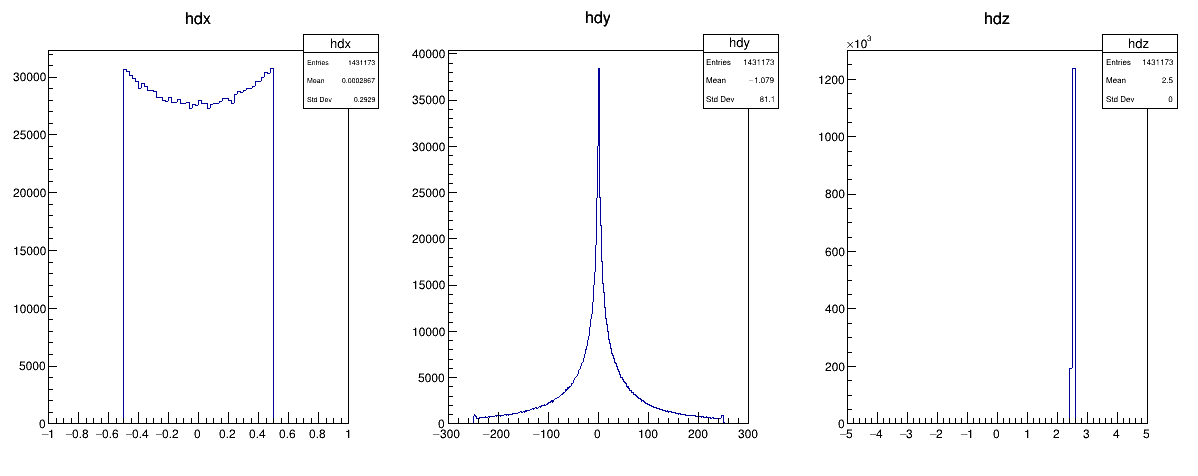
\includegraphics[width=\textwidth]{check_pos.png}
  \end{figure}
  \href{https://github.com/MegMev/k4megat/blob/sim-dev/analysis/scripts/demo_tpc_pos.C}{https://github.com/MegMev/k4megat/blob/sim-dev/analysis/scripts/demo\_tpc\_pos.C}
\end{frame}
\end{document}

%%% Local Variables:
%%% TeX-command-extra-options: "-shell-escape"
%%% End:
